\documentclass[12pt,a4paper]{article}
% Packages for enhanced functionality
\usepackage[utf8]{inputenc}
\usepackage[T1]{fontenc}
\usepackage{graphicx} % For including images
\usepackage{geometry} % For page layout
\usepackage{hyperref} % For clickable links and references
\usepackage{fancyhdr} % For custom headers and footers
\usepackage{float} 
\usepackage{circuitikz}
\usepackage{caption}
\usepackage{graphicx}
\usepackage{subcaption}
\usepackage{hyperref}
\usepackage{siunitx}
\usepackage{amsmath}
\usepackage{tikz}
\usepackage{subcaption}
\usepackage{booktabs}
\newcommand{\vecb}[1]{\mathbf{#1}}
\newcommand{\brak}[1]{\ensuremath{\left(#1\right)}}
\newcommand{\cbrak}[1]{\ensuremath{\left\{#1\right\}}}
\newcommand{\abs}[1]{\left\vert#1\right\vert}
\newcommand{\norm}[1]{\left\lVert#1\right\rVert}
\providecommand{\sbrak}[1]{\ensuremath{{}\left[#1\right]}}
\providecommand{\lsbrak}[1]{\ensuremath{{}\left[#1\right.}}
\providecommand{\rsbrak}[1]{\ensuremath{{}\left.#1\right]}}
\providecommand{\brak}[1]{\ensuremath{\left(#1\right)}}
\providecommand{\lbrak}[1]{\ensuremath{\left(#1\right.}}
\providecommand{\rbrak}[1]{\ensuremath{\left.#1\right)}}
\providecommand{\cbrak}[1]{\ensuremath{\left\{#1\right\}}}
\providecommand{\lcbrak}[1]{\ensuremath{\left\{#1\right.}}
\providecommand{\rcbrak}[1]{\ensuremath{\left.#1\right\}}}
\hypersetup{
    colorlinks=true,  % Enable colored text links
    linkcolor=orange,    % Internal links (sections, table of contents, etc.)
    urlcolor=orange,     % External URLs
    citecolor=orange,    % Citations
    pdfborder={0 0 0} % Remove ugly default borders
}


\title{\textbf{Lab Report: Experiment 5}}
\author{EE24BTECH11003 : Akshara Sarma Chennubhatla\\EE24BTECH11005 : Arjun Pavanje}

\begin{document}
\maketitle
\begin{center}
	\textbf{Experiment:\\}Measuring the I-V characteristics\\of a diode and determining\\Is and n. Finding small signal dynamic\\resistance(rd). Analyzing the\\DTFT of Id and determining\\harmonic amplitudes.
\end{center}
\vspace{30pt}
\begin{figure}[h!]
	\centering
	
\includegraphics[width = 100pt]{logo.png}\\
\end{figure}
\begin{center}
	Bachelor of Technology\\
	\vspace{10pt}
	Department of Electrical Engineering\\
\end{center}
\newpage


\section{Aim}
\begin{enumerate}
\item Measure the DC I–V characteristic of a diode and extract diode parameters (ideality factor $\mathbf{\eta}$ and saturation current $\mathbf{I_s}$). 
\item Measure the small-signal (dynamic) resistance $\mathbf{r_d}$ around a chosen bias point and verify the small-signal model. 
\item Further, bias the diode with a DC voltage and apply a small AC signal. Observe the output on the CRO and use FFT mode to see harmonics. The diode current is nonlinear,
\begin{align*}
I \approx I_0 + g_1v + \frac{1}{2}g_2*v^2.
\end{align*}
\begin{itemize}
\item For small $V_{ac}$, only the fundamental appears. 
\item As $V_{ac}$ increases, 2nd and higher harmonics appear, showing nonlinearity. 
\item Measure fundamental and 2nd harmonic amplitudes vs $V_{ac}$ and note slopes $~1$ and $~2$
\end{itemize}
\end{enumerate}

\section{I-V characteristics of Diode}
$V_D$ (diode voltage) is calculated for multiple values of $V_S$ (source voltage). The below circuit is used, along with a multimeter to take voltage readings for multiple $V_S$ values
\begin{figure}[!ht]
\centering
\resizebox{0.5\textwidth}{!}{%
\begin{circuitikz}
\tikzstyle{every node}=[font=\normalsize]
\draw (3.75,12.5) to[american voltage source,l={ \normalsize $V_S$}] (3.75,10);
\draw (3.75,12.5) to[R,l={ \normalsize R}] (6.25,12.5);
\draw (6.25,12.5) to[D,l={ \normalsize 1N4007}] (6.25,10);
\draw (6.25,10) to[short] (3.75,10);
\end{circuitikz}
}%
\end{figure}
\pagebreak
\begin{table}[h!]
\centering
\begin{tabular}{|c|c|}
\hline
$V_S$ (V) & $V_D$ (V) \\
\hline
0.0 & 0.0 \\
0.1 & 0.143 \\
0.2 & 0.250 \\
0.4 & 0.399 \\
0.6 & 0.478 \\
0.8 & 0.519 \\
1.0 & 0.544 \\
1.2 & 0.560 \\
1.4 & 0.571 \\
1.6 & 0.579 \\
1.8 & 0.588 \\
2.0 & 0.595 \\
2.2 & 0.601 \\
2.4 & 0.608 \\
2.6 & 0.614 \\
2.8 & 0.617 \\
3.0 & 0.621 \\
3.2 & 0.626 \\
3.4 & 0.629 \\
3.6 & 0.633 \\
3.8 & 0.636 \\
4.0 & 0.639 \\
4.2 & 0.641 \\
4.4 & 0.644 \\
4.6 & 0.647 \\
4.8 & 0.649 \\
5.0 & 0.652 \\
\hline
\end{tabular}
\end{table}
\newline We require the exponential curve that is closest to all the obtained data points. So curve-fitting must be done. Scipy's curve$\_$fit was used. $I_s, \eta$ was calculated using the same python code.\\
Schokley's equation for the diode was used for curve fitting with parameters $I_S, \eta$.
\begin{align*}
    I_D = I_S(e^{\frac{V_D}{\eta V_T}} - 1)
\end{align*}
\pagebreak
\begin{figure}[h!]
\centering
\begin{subfigure}[b]{0.47\linewidth}
    \centering
    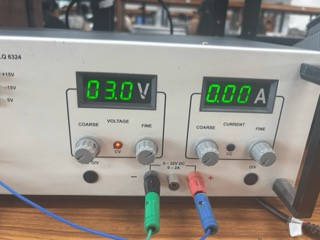
\includegraphics[width=\textwidth]{Experiment_5/figs/iv_dc_1 Small.jpeg}
    \caption{Input $V_S$}
\end{subfigure}
\begin{subfigure}[b]{0.48\linewidth}
    \centering
    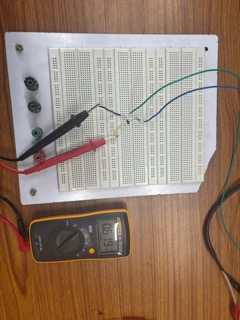
\includegraphics[angle=90, width=\textwidth]{Experiment_5/figs/iv_ckt_1 Small.jpeg}
    \caption{Output $V_D$}
\end{subfigure}
\end{figure}
\begin{figure}[h!]
\centering
\begin{subfigure}[b]{0.47\linewidth}
    \centering
    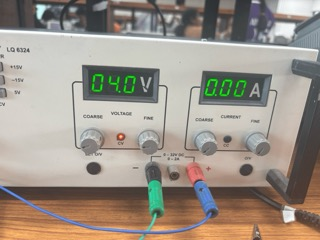
\includegraphics[width=\textwidth]{Experiment_5/figs/iv_dc_2 Small.jpeg}
    \caption{Input $V_S$}
\end{subfigure}
\begin{subfigure}[b]{0.48\linewidth}
    \centering
    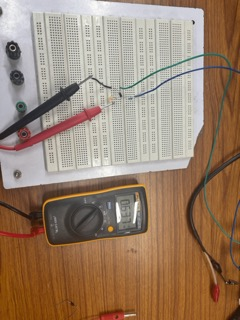
\includegraphics[angle=90, width=\textwidth]{Experiment_5/figs/iv_ckt_2 Small.jpeg}
    \caption{Output $V_D$}
\end{subfigure}
\end{figure}
\begin{figure}[h!]
\centering
\begin{subfigure}[b]{0.47\linewidth}
    \centering
    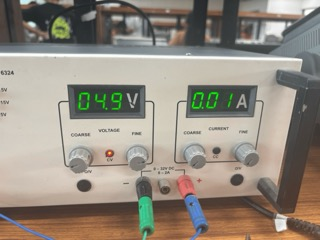
\includegraphics[width=\textwidth]{Experiment_5/figs/iv_dc_3 Small.jpeg}
    \caption{Input $V_S$}
\end{subfigure}
\begin{subfigure}[b]{0.48\linewidth}
    \centering
    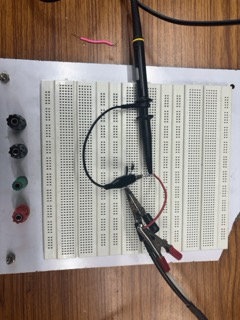
\includegraphics[angle=90, width=\textwidth]{Experiment_5/figs/iv_ckt_3 Small.jpeg}
    \caption{Output $V_D$}
\end{subfigure}
\end{figure}
\pagebreak
\newline Curve ($I_S$ vs $V_D$) obtained through curve-fitting
\begin{figure}[h!]
    \centering
    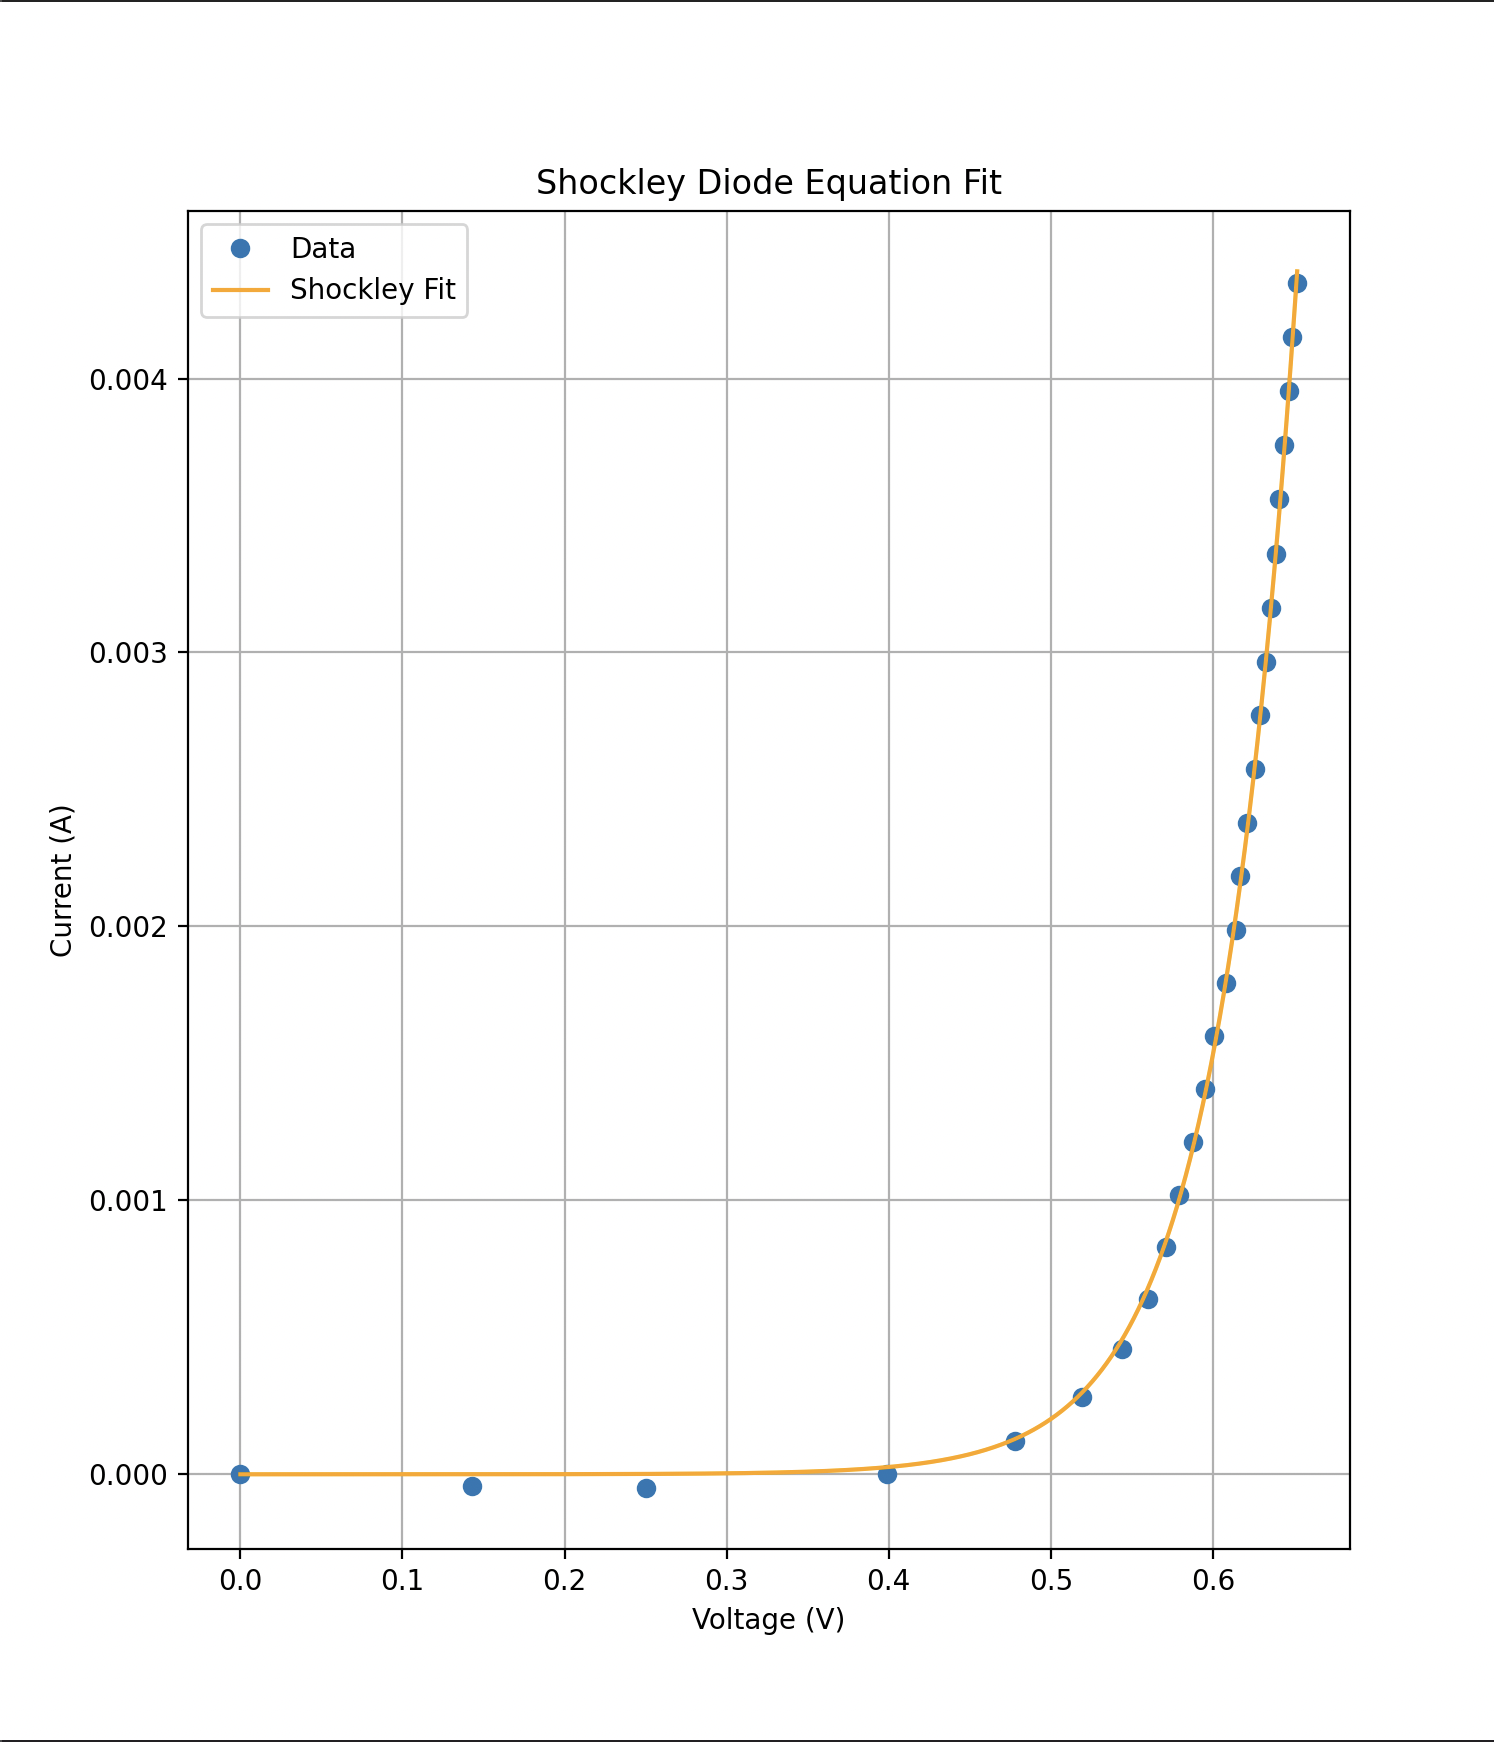
\includegraphics[width=0.7\linewidth]{figs/curve_fit.png}
\end{figure}
\newline We obtain diode parameters,
\begin{itemize}
    \item Ideality factor ($\eta$) = $1.907$
    \item Saturation current ($I_s$) = $8.109nA$
\end{itemize}
Code used for curve-fitting can be found at, \url{https://github.com/ArjunPavanje/EE2301/blob/main/Experiment_5/codes/diode.py}
\pagebreak
\section{Small Signal Analysis}
After fixing a bias point, a sine-wave of very small amplitude was applied to calculate small signal characteristics.
\begin{figure}[!ht]
\centering
\resizebox{0.6\textwidth}{!}{%
\begin{circuitikz}
\tikzstyle{every node}=[font=\normalsize]
\draw (3.75,12.5) to[american voltage source,l={ \normalsize $V_s$}] (3.75,10);
\draw (3.75,12.5) to[R,l={ \normalsize R}] (6.25,12.5);
\draw (6.25,12.5) to[D,l={ \normalsize 1N4007}] (6.25,10);
\draw (3.75,10) to[sinusoidal voltage source, sources/symbol/rotate=auto,l={ \normalsize $V_{ac}$}] (6.25,10);
\end{circuitikz}
}%
\end{figure}
\newline We pick 2 points and note $V_S, V_D$ values.
\begin{figure}[ht!]
\centering
\begin{subfigure}[b]{0.47\linewidth}
    \centering
    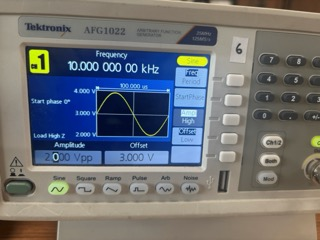
\includegraphics[width=\textwidth]{Experiment_5/figs/rd_osc Small.jpeg}
    \caption{Function generator input}
\end{subfigure}
\begin{subfigure}[b]{0.48\linewidth}
    \centering
    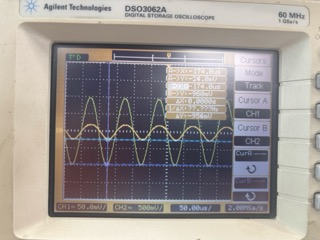
\includegraphics[width=\textwidth]{Experiment_5/figs/rd Small.jpeg}
    \caption{Oscilloscope output}
\end{subfigure}
\end{figure}
\begin{table}[h!]
\centering
\begin{tabular}{|c|c|}
\hline
$V_s$ & $V_d$ \\
\hline
3.960 & 3.018 \\
2.040 & 2.982 \\
\hline
\end{tabular}
\end{table}
\newline Small signal parameter $r_d$ is calculated (for bias point $V_D = 3V$) as,
\begin{align*}
    r_d &= \left(\frac{dI_D}{dV_D}\right)^{-1} = \frac{d}{dV_D}(I_S(e^{\frac{V_D}{\eta V_T}} - 1))\\
    r_d &= \frac{\eta V_T}{I_D + I_S}\\
    r_d &\approx \frac{\eta V_T}{I_D}
\end{align*}

\begin{itemize}
    \item Theoretical: $\frac{\eta V_T}{I_D} = 20.69782927852349\Omega$
    \item Calculated: $\frac{\Delta V_D}{\Delta I_D} = 19.108280254776847\Omega$
\end{itemize}
$I_D$ is found by $\frac{V_S - V_D}{R}$. $\eta$ value calculated previously is used in theoretical calculation. Thus, small signal parameter $r_d$ is calculated and verified.
Code used to calculate and verify small signal parameter ($r_d$) can be found at, \url{https://github.com/ArjunPavanje/EE2301/blob/main/Experiment_5/codes/rd.py}
\section{FFT Harmonics}
To observe FFT harmonics we reuse the circuit built previously,
\begin{figure}[!ht]
\centering
\resizebox{0.6\textwidth}{!}{%
\begin{circuitikz}
\tikzstyle{every node}=[font=\normalsize]
\draw (3.75,12.5) to[american voltage source,l={ \normalsize $V_s$}] (3.75,10);
\draw (3.75,12.5) to[R,l={ \normalsize R}] (6.25,12.5);
\draw (6.25,12.5) to[D,l={ \normalsize 1N4007}] (6.25,10);
\draw (3.75,10) to[sinusoidal voltage source, sources/symbol/rotate=auto,l={ \normalsize $V_{ac}$}] (6.25,10);
\end{circuitikz}
}%
\end{figure}
\newline To observe harmonics of $I_D$ we can just observe resistor voltage ($V_S-V_D$) as it is just a scaled version ($RI_D$) of diode current. When $V_{ac}$ is very small, we observe only one peak at frequency $f$ (frequency of sinusoidal signal). As we increase $V_{ac}$, number of peaks increases and the peaks occur at $f, 2f, 3f, \cdots$.\\\\
This happens due to the fact that the DTFT of a sinusoidal wave has a single peak at the fundamental frequency of the wave. Now as we expand $I_D$ using taylor series, we get:
\begin{align*}
    WKT,\\
    I_D &= I_S(e^{\frac{V_D}{\eta V_T}} - 1)\\
    Also,\\
    I_{D0} &= I_S(e^{\frac{V_{D0}}{\eta V_T}} - 1)
\end{align*}
Since, the input signal is a sinusoidal small signal with a DC offset, we can write:
\begin{align*}
    V_D = V_{D0} + v(t)
\end{align*}
Substituing this in the previous equation:
\begin{align*}
    I_D &= I_S(e^{\frac{(V_{D0} + v(t))}{\eta V_T}} - 1)\\
    I_D &= I_S(e^{\frac{v(t)}{\eta V_T}}(\frac{I_{D0}}{I_S} + 1) - 1)\\
    I_D &= I_{D0} + I_Se^{\frac{V_{D0}}{\eta V_T}}(e^{\frac{v(t)}{\eta V_T}} - 1)\\
\end{align*}
Expanding Taylor series for $e^{\frac{v(t)}{\eta V_T}}$,
\begin{align*}
e^{\frac{V_{D0} + v(t)}{\eta V_T}}
&= e^{\frac{V_{D0}}{\eta V_T}} \, e^{\frac{v(t)}{\eta V_T}} \\[6pt]
&= e^{\frac{V_{D0}}{\eta V_T}}
\left[
1
+ \frac{v(t)}{\eta V_T}
+ \frac{1}{2!}\left(\frac{v(t)}{\eta V_T}\right)^2
+ \frac{1}{3!}\left(\frac{v(t)}{\eta V_T}\right)^3
+ \frac{1}{4!}\left(\frac{v(t)}{\eta V_T}\right)^4
+ \cdots
\right]
\end{align*}
So $I_D$ becomes,
\begin{align*}
    I_D &= I_{D0} + I_S e^{\frac{V_{D0}}{\eta V_T}}\left[ \frac{v(t)}{\eta V_T}
+ \frac{1}{2!}\left(\frac{v(t)}{\eta V_T}\right)^2
+ \frac{1}{3!}\left(\frac{v(t)}{\eta V_T}\right)^3
+ \frac{1}{4!}\left(\frac{v(t)}{\eta V_T}\right)^4
+ \cdots \right]\\
I_D &= I_{D0} + \left(\frac{I_S e^{\frac{V_{D0}}{\eta V_T}}}{\eta V_T}\right)v(t)
+ \frac{1}{2}\left(\frac{I_S e^{\frac{V_{D0}}{\eta V_T}}}{(\eta V_T)^2}\right)v(t)^2 + \cdots
\end{align*}
Taking $g_1 = \frac{I_S e^{\frac{V_{D0}}{\eta V_T}}}{\eta V_T}$ and $g_2 = \frac{I_S e^{\frac{V_{D0}}{\eta V_T}}}{(\eta V_T)^2}$,
\begin{align*}
    I_D &= I_{D0} + g_1v(t) + \frac{1}{2}g_2v(t)^2 + \cdots\\
    \implies I_D &\approx I_{D0} + g_1v(t) + \frac{1}{2}g_2v(t)^2
\end{align*}
Since terms like $v(t), v(t)^2,...$ are present, and the v(t) is a sum of sines in itself, we get sum of sines of different frequencies, all being the multiples of the fundamental frequency of the input sine wave. So we get peaks at every multiple of input frequency due to the fact that $I_D$ is a sum of sines.

\subsection*{Harmonic Amplitudes:}

At small $v(t)$ values, we can neglect all the other terms in the Taylor series expansion of $I_D$ except the fundamental and the first harmonic. At this small $v(t)$, we can consider it to be just a simple sinusoidal signal which is a scaled down version of the input signal.\\\\
The amplitude of $v(t)$ can be written as:
\begin{align*}
    A = V_m\frac{r_d}{r_d + R_L}
\end{align*}
where $V_m$ is the amplitude of the input sine signal. So, applying this in the equation,
\begin{align*}
    I_D = I_{D0} + g_1Asin(2 \pi f t)
\end{align*}
where $f$ is the frequency of the input sine wave.\\
So the first peak occurs at $f$ with amplitude $g_1A$. By plugging in the values, we get
\begin{align*}
    \text{Amplitude} = 4.993 \times 10^{-4}
\end{align*}
When we increase $V_m$ by a bit such that the second harmonic also is seen, $I_D$ can be written as:
\begin{align*}
     I_D &= I_{D0} + g_1Asin(2 \pi f t) + \frac{1}{2}g_2A^2sin^2(2\pi ft)\\
     I_D &= I_{D0} + g_1Asin(2 \pi f t) + \frac{1}{2}g_2A^2(1 - cos(4\pi ft))
\end{align*}
So, the second peak occurs at $2f$ with amplitude $\frac{1}{2}g_2A^2$. By plugging in the values, we get
\begin{align*}
    \text{Amplitude} = 15.96 \times 10^{-4}
\end{align*}
\pagebreak
\subsection*{Interpretation of Slopes for Fundamental and Second Harmonic}

When we plot the amplitudes of the fundamental and second harmonic components of the diode current 
with respect to the amplitude of the applied AC voltage $V_{\text{ac}}$ on a log–log scale, we observe 
different slopes corresponding to the order of nonlinearity.

For small signal amplitudes, the diode current can be expressed as
\[
I_D(t) = I_{D0} + g_1 v(t) + \frac{1}{2}g_2 v(t)^2 + \cdots
\]
where $v(t) = V_m \sin(\omega t)$.

The amplitude of the fundamental component is proportional to $V_m$, i.e.,
\[
I_{\text{fundamental}} \propto V_m
\]
and the amplitude of the second harmonic component is proportional to $V_m^2$, i.e.,
\[
I_{\text{2nd harmonic}} \propto V_m^2
\]

Therefore, when plotting $\log(I_{\text{fundamental}})$ and $\log(I_{\text{2nd harmonic}})$ versus 
$\log(V_{\text{ac}})$:

\[
\text{slope of fundamental} \approx 1, \quad
\text{slope of 2nd harmonic} \approx 2
\]

This indicates that the fundamental component arises from the first-order (linear) term, while 
the second harmonic arises from the second-order (nonlinear) term in the diode’s exponential I–V characteristic.

Below are the pictures of the FFT mode on the oscilloscope for increasing $V_m$ values:

\begin{figure}[h!]
\centering
\begin{subfigure}[b]{0.47\linewidth}
    \centering
    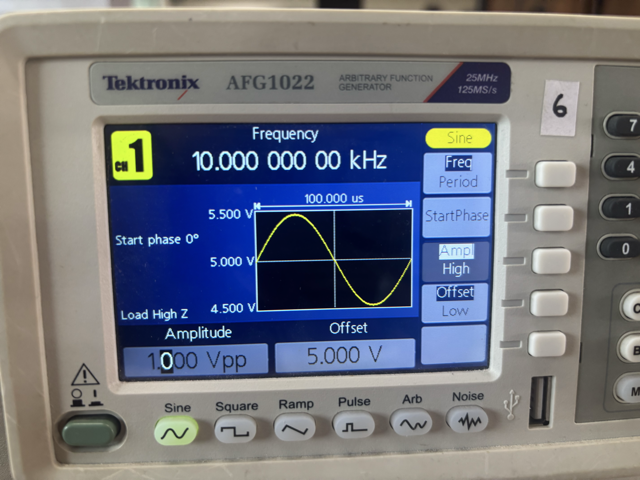
\includegraphics[width=\textwidth]{Experiment_5/figs/FFT_gen_1.png}
    \caption{Function generator}
\end{subfigure}
\begin{subfigure}[b]{0.48\linewidth}
    \centering
    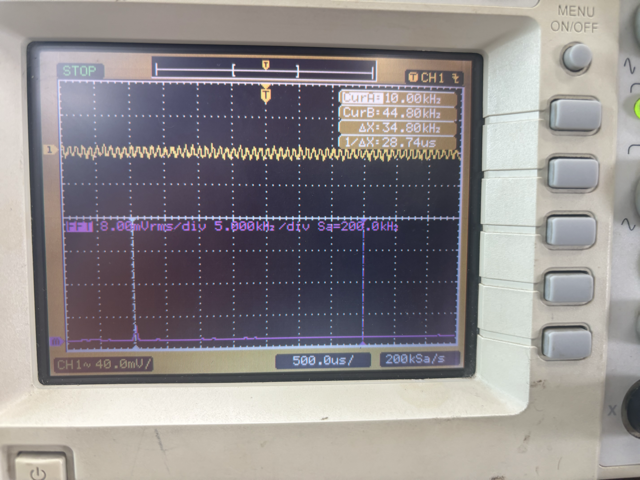
\includegraphics[width=\textwidth]{Experiment_5/figs/FFT_osc_1.png}
    \caption{Oscilloscope}
\end{subfigure}
\end{figure}
\pagebreak
\begin{figure}[h!]
\centering
\begin{subfigure}[b]{0.47\linewidth}
    \centering
    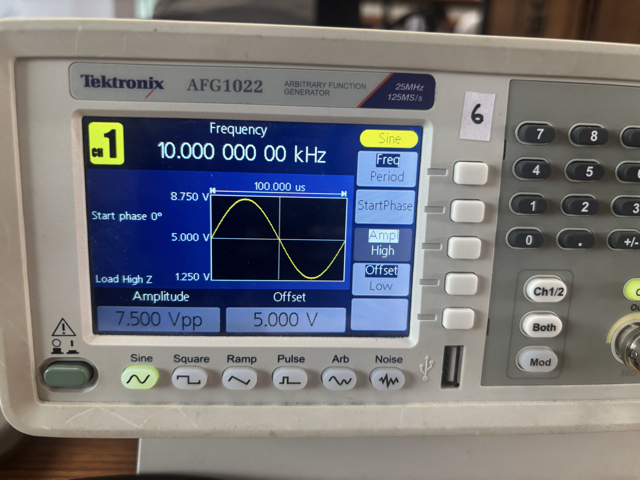
\includegraphics[width=\textwidth]{Experiment_5/figs/FFT_gen_2.png}
    \caption{Function generator}
\end{subfigure}
\begin{subfigure}[b]{0.48\linewidth}
    \centering
    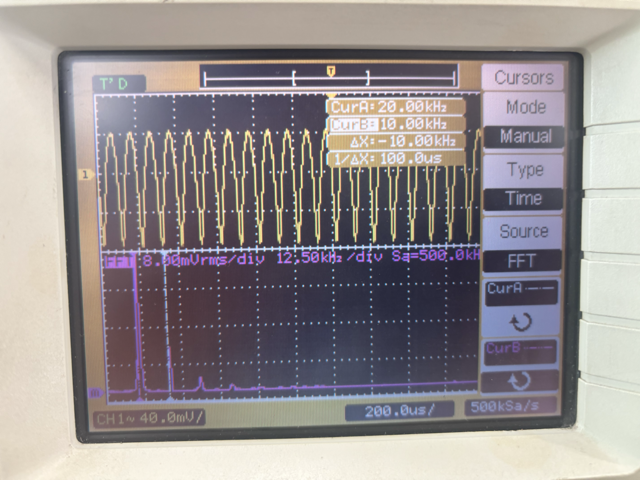
\includegraphics[width=\textwidth]{Experiment_5/figs/FFT_osc_2.png}
    \caption{Oscilloscope}
\end{subfigure}
\end{figure}
\begin{figure}[h!]
\centering
\begin{subfigure}[b]{0.47\linewidth}
    \centering
    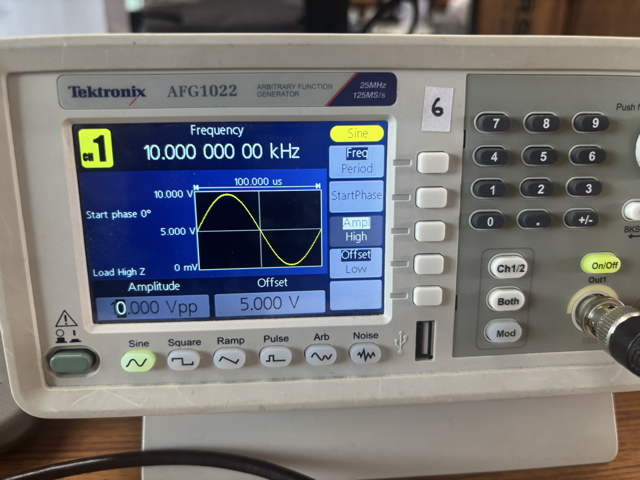
\includegraphics[width=\textwidth]{Experiment_5/figs/FFT_gen_3.png}
    \caption{Function generator}
\end{subfigure}
\begin{subfigure}[b]{0.48\linewidth}
    \centering
    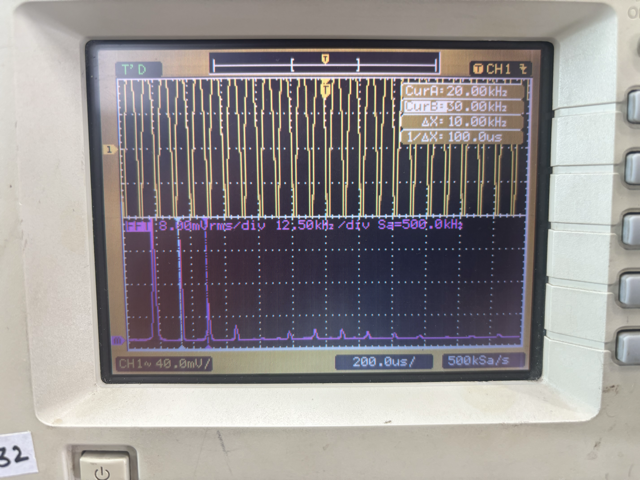
\includegraphics[width=\textwidth]{Experiment_5/figs/FFT_osc_3.png}
    \caption{Oscilloscope}
\end{subfigure}
\end{figure}
\begin{figure}[h!]
\centering
\begin{subfigure}[b]{0.47\linewidth}
    \centering
    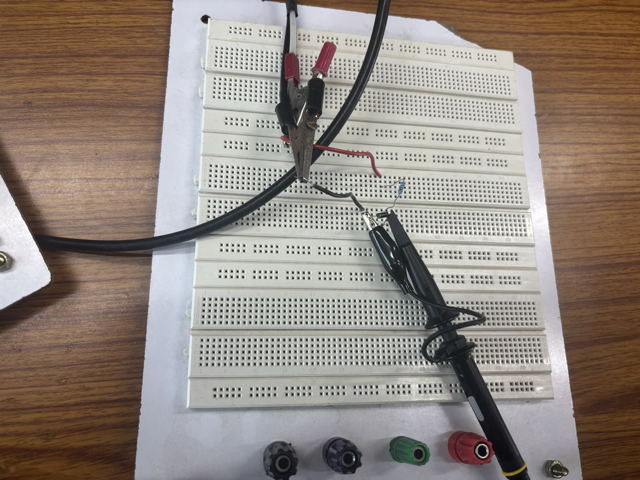
\includegraphics[width=\textwidth]{Experiment_5/figs/FFT_ckt.png}
\end{subfigure}
\begin{subfigure}[b]{0.48\linewidth}
    \centering
    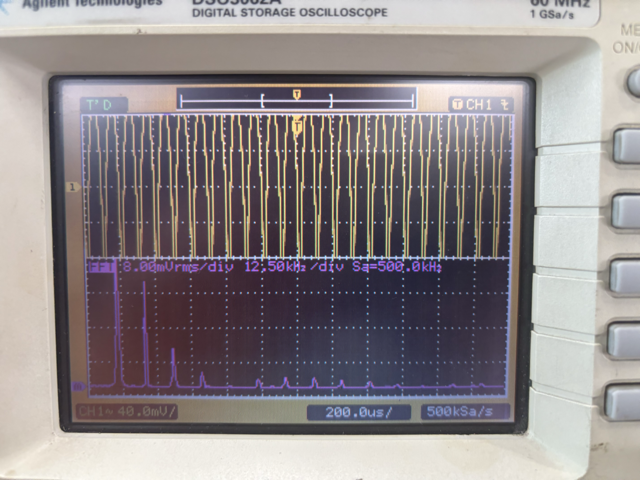
\includegraphics[width=\textwidth]{Experiment_5/figs/FFT_osc.png}
\end{subfigure}
\end{figure}
Code used to calculate amplitudes can be found at, \url{https://github.com/ArjunPavanje/EE2301/blob/main/Experiment_5/codes/fft.py}
\section{Conclusion}
In this experiment, I-V characteristics of diodes were plotted and diode parameters $I_S$ (saturation current), $\eta$ (ideality factor) were found. Next, by giving a small AC-signal at a particular bias point, we estimate small signal parameter $r_d$ and verified it. Finally, using FFT mode, harmonics in diode current were observed by adjusting values of $V_{ac}$.
\end{document}